\documentclass[]{article}
\usepackage{lmodern}
\usepackage{amssymb,amsmath}
\usepackage{ifxetex,ifluatex}
\usepackage{fixltx2e} % provides \textsubscript
\ifnum 0\ifxetex 1\fi\ifluatex 1\fi=0 % if pdftex
  \usepackage[T1]{fontenc}
  \usepackage[utf8]{inputenc}
\else % if luatex or xelatex
  \ifxetex
    \usepackage{mathspec}
  \else
    \usepackage{fontspec}
  \fi
  \defaultfontfeatures{Ligatures=TeX,Scale=MatchLowercase}
\fi
% use upquote if available, for straight quotes in verbatim environments
\IfFileExists{upquote.sty}{\usepackage{upquote}}{}
% use microtype if available
\IfFileExists{microtype.sty}{%
\usepackage{microtype}
\UseMicrotypeSet[protrusion]{basicmath} % disable protrusion for tt fonts
}{}
\usepackage[margin=1in]{geometry}
\usepackage{hyperref}
\hypersetup{unicode=true,
            pdftitle={Analyse de données},
            pdfborder={0 0 0},
            breaklinks=true}
\urlstyle{same}  % don't use monospace font for urls
\usepackage{graphicx,grffile}
\makeatletter
\def\maxwidth{\ifdim\Gin@nat@width>\linewidth\linewidth\else\Gin@nat@width\fi}
\def\maxheight{\ifdim\Gin@nat@height>\textheight\textheight\else\Gin@nat@height\fi}
\makeatother
% Scale images if necessary, so that they will not overflow the page
% margins by default, and it is still possible to overwrite the defaults
% using explicit options in \includegraphics[width, height, ...]{}
\setkeys{Gin}{width=\maxwidth,height=\maxheight,keepaspectratio}
\IfFileExists{parskip.sty}{%
\usepackage{parskip}
}{% else
\setlength{\parindent}{0pt}
\setlength{\parskip}{6pt plus 2pt minus 1pt}
}
\setlength{\emergencystretch}{3em}  % prevent overfull lines
\providecommand{\tightlist}{%
  \setlength{\itemsep}{0pt}\setlength{\parskip}{0pt}}
\setcounter{secnumdepth}{0}
% Redefines (sub)paragraphs to behave more like sections
\ifx\paragraph\undefined\else
\let\oldparagraph\paragraph
\renewcommand{\paragraph}[1]{\oldparagraph{#1}\mbox{}}
\fi
\ifx\subparagraph\undefined\else
\let\oldsubparagraph\subparagraph
\renewcommand{\subparagraph}[1]{\oldsubparagraph{#1}\mbox{}}
\fi

%%% Use protect on footnotes to avoid problems with footnotes in titles
\let\rmarkdownfootnote\footnote%
\def\footnote{\protect\rmarkdownfootnote}

%%% Change title format to be more compact
\usepackage{titling}

% Create subtitle command for use in maketitle
\providecommand{\subtitle}[1]{
  \posttitle{
    \begin{center}\large#1\end{center}
    }
}

\setlength{\droptitle}{-2em}

  \title{Analyse de données}
    \pretitle{\vspace{\droptitle}\centering\huge}
  \posttitle{\par}
    \author{}
    \preauthor{}\postauthor{}
    \date{}
    \predate{}\postdate{}
  

\begin{document}
\maketitle

\hypertarget{introduction}{%
\subsection{Introduction}\label{introduction}}

Notre jeu de données présente 40 patients. Les 20 premiers sont en
bonnes santés alors que les autres sont gravements malades. Les patients
sont représentés en colonnes et les gênes sont représentés.

Nous savons qu'il existe de nombreuses maladies dues l'expression des
gênes. On en dénombre entre 6000 et 8000 maladies génétiques dans le
mondes. Leurs causes ainsi que leurs symptômes sont diverses en variés.
Ses maladies peuvent être héréditaires ou simplement dues à des
mutatations génétiques dans la vie adulte. Ainsi la modification d'un
gêne peut provoquer des protéines déficientes et le fonctionnement
anormal de nombreuses cellules. Dans 80\% des cas, un maladie
génétiquesserait due à l'altération d'une séquence codante d'un gêne. Le
but de notre études est de trouver les gênes ou les groupes responsables
des maladies sur nos patients par une analyse en composante principale.
This is an R Markdown document. Markdown is a simple formatting syntax
for authoring HTML, PDF, and MS Word documents.

\hypertarget{description-des-individus}{%
\subsection{Description des individus}\label{description-des-individus}}

Sur nos quarantes, nous remarquons que chaque individu a des gênes qui
s'expriments plus que d'autres et d'autres qui s'expriment mois bien.
Sur le graphique nos pouvons que ces gênes sont mis en avant par leurs
valeurs atypiques qui se retrouvent aux extrémités des boîtes à
moustache.

\begin{center}\includegraphics[width=1\linewidth,height=1\textheight]{C:/Users/viche/Pictures/gene} \end{center}

Cependant, l'expression des gènes chez les individus sains diffèrent de
leurs expressions par rapport aux individus qui sont malades.

\begin{center}\includegraphics[width=1\linewidth,height=1\textheight]{C:/Users/viche/Pictures/boxplotsains} \end{center}

En effet nous pouvous remarquer que nous avons quasiment autant de gênes
qui sont sur-exprimés et sous exprimés chez les individus sains. Alors
que pour les individus malades nous avons beaucoups plus de gènes qui
sont sur-exprimés comme le montre l'image ci-dessous.

\begin{center}\includegraphics[width=1\linewidth,height=1\textheight]{C:/Users/viche/Pictures/boxplotmalade} \end{center}

C'est pour cela que les boites à moustaches des individus malades ont
une médiane tirée vers le haut par rapport aux individus sains.

Nous pouvons premièrement conlure que les deux groupes d'individus sont
alors différenciés par certains gènes. Nous allons essayer de décrire
ces gènes par la suite.

\hypertarget{description-des-guxe8nes}{%
\subsection{Description des gènes}\label{description-des-guxe8nes}}

Ici nous pouvons remarquer que la distribution de l'expression est
étendue de 1 à 4.

\begin{center}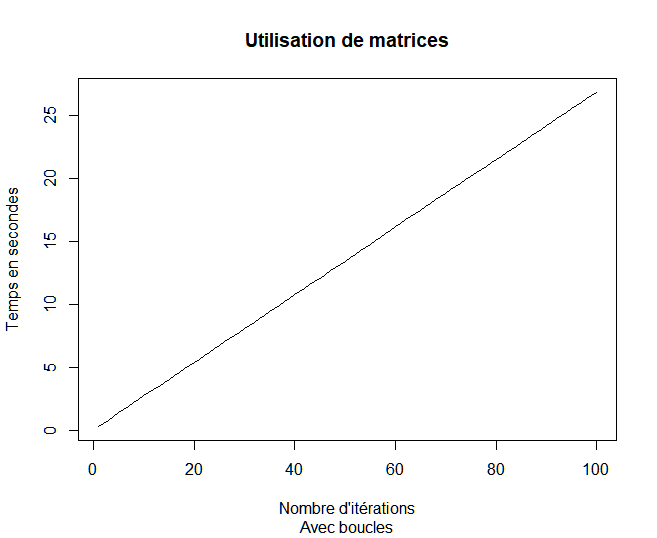
\includegraphics[width=1\linewidth,height=1\textheight]{C:/Users/viche/Pictures/Rplot01} \end{center}

Nous pouvons supposer à première vue que que l'expression des gènes est
distribuer selon une loi Gaussienne qui donne une bonne répartition de
la distribution par rapport à la distribution des gènes des individus
malades ci-dessous.

\begin{center}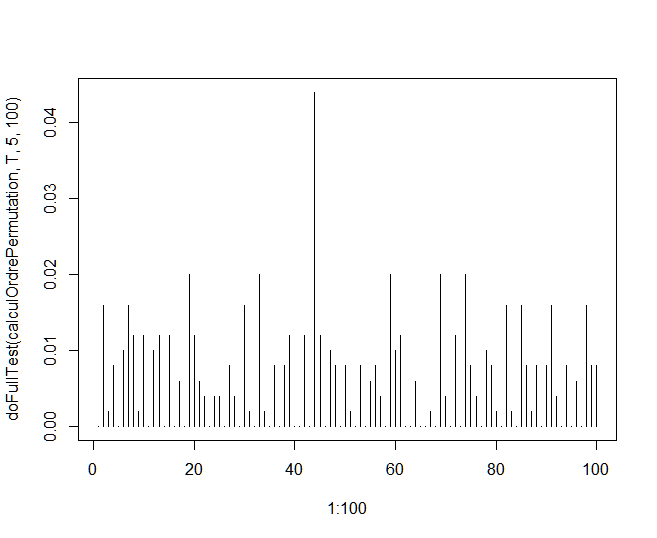
\includegraphics[width=1\linewidth,height=1\textheight]{C:/Users/viche/Pictures/Rplot02} \end{center}

Nous remarquon alors que la distribution des gênes n'est pas la même
lorqu'un individus est malade. C'est pour cela que nous pensons que les
maladies peuvent être dûs à la sous-expression ou sur-expression de
certains gênes. L'ACP pourrait alors nous être utiles pour retrouver les
gênes et faire les groupes d'individus.

\hypertarget{lacp}{%
\subsection{L'ACP}\label{lacp}}

Nous avons commencé à faire une ACP sur notre tous nos variables en même
temps. Cependant, l'inertie de nos points se retrouvent au centre de
notre cercle de corrélation et nos axes factorielles ne représentent pas
bien la réalité de notre études.

Cela est précisé par le graphique des valeurs propres où seule la
prmière valeur propre explique nos données de l'étude de avec la règle
du coude

\begin{center}\includegraphics[width=1\linewidth,height=1\textheight]{C:/Users/viche/Pictures/dimACP} \end{center}

Les autres inerties étant trop faible, la projection de nos 1000 gênes
sur le cercle de corrélation n'est pas cohérente avec notre étude.


\end{document}
